\section{Building the corpus of regexes}
\label{sec:corpusBuilding}

The goal of this experiment was to collect regexes from a variety of projects to represent the breadth of how developers use the language features.

\subsection{Selecting projects to mine for utilizations}
Using the GitHub API, \dbfetch{nProjScanned} projects containing Python code were mined for utilizations as described in Section~\ref{sec:miningImplementation}.  This section describes how these projects were selected.

Every time a new repository is created on Github, a new unique identifier (strictly greater than existing identifiers) is generated and assigned to that repository.  This work refers to these identifiers using the shorthand: \emph{repo ID}.  At the time the mining for utilizations used in this study was performed, the largest repo ID was between 32 million and 33 million.  Dividing these repo IDs into four groups each of size $2^23 = 8,388,608$ (with the fourth group being a little larger than that), the second group, which spans the range 8,388,608 - 16,777,215 was split into 32 sections so that starting indices were 262,144 repo IDs apart.  The original intention was to mine the entire second $1/4$ of the first 32 million repo IDs, but due to the challenges described in Section~\ref{sec:miningChallenges}, only the first 100 or so projects from each of the 32 starting points was mined.  Instead of spending the majority of available time on perfecting a mining technique, the determination was made to analyze the data that had already been gathered.

\begin{table}[tb]
\begin{center}
\begin{small}
\caption{How saturated are projects with utilizations? (RQ2)}
\label{table:saturation}

\begin{tabular}{l|ccccc}
\toprule
source & Q1 & Avg & Med & Q3 & Max \\
 \midrule \bigstrut
utilizations per project & 2 & 32 & 5 & 19 & 1,427 \\
 \midrule \bigstrut
files per project & 2 & 53 & 6 & 21 & 5,963 \\
 \midrule \bigstrut
utilizing files per project & 1 & 11 & 2 & 6 & 541 \\
 \midrule \bigstrut
utilizations per file & 1 & 2 & 1 & 3 & 207 \\
\bottomrule
\end{tabular}
\end{small}
\end{center}
\vspace{-12pt}
\end{table}


\subsection{Saturation}
Out of the \dbfetch{nProjScanned}\ projects scanned, \dbfetch{percentProjectsUsingRegex}\% (\dbfetch{nProjectsUsingRegex}) contained at least one utilization.  Within a project, a duplicate utilization was marked when two versions of the same file have the same function, pattern and flags.  In total, \dbfetch{nUsages} non-duplicate utilizations were observed.  To illustrate how saturated projects are with regexes, measurements are made for the number of utilizations per project, number of files scanned per project, number of files containing utilizations, and number of utilizations  per file, as shown in Table~\ref{table:saturation}.

Of projects containing at least one utilization, the average utilizations per project was 32 and the maximum  was 1,427.  The project with the most utilizations is a C\# project\footurl{https://github.com/Ouroboros/Arianrhod} that maintains a collection of source code for 20 Python libraries, including larger libraries like {\tt pip}, {\tt celery} and {\tt ipython}.  These larger Python libraries contain many utilizations.
From Table~\ref{table:saturation}, it can also be seen that each project had an average of 11 files containing any utilization, and each of these files had an average of 2 utilizations.

\begin{figure}[tb]
\centering
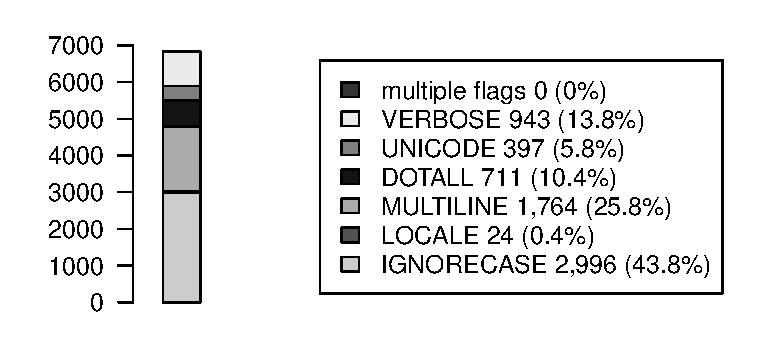
\includegraphics[width=0.9\columnwidth]{nontex/illustrations/partFlags.eps}
\vspace{-6pt}
\caption{Which behavioral flags are used?}
\vspace{-6pt}
\label{fig:partFlags}
\end{figure}

\begin{figure}[tb]
\centering
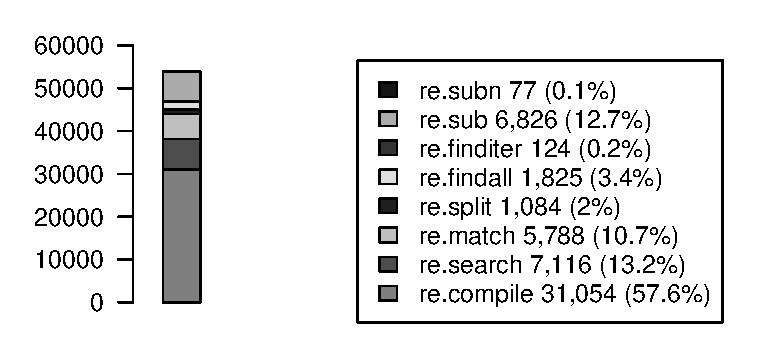
\includegraphics[width=\columnwidth]{nontex/illustrations/partFunctions.eps}
\vspace{-12pt}
\caption{How often are  {\tt re} functions used?}
\vspace{-6pt}
\label{fig:partFunctions}
\end{figure}

\subsection{Flags and functions}
As shown in figure ~\ref{fig:partFlags}, of all behavioral flags used, ignorecase (\DTLfetch{data}{key}{percentI}{value}\%) and multiline (\DTLfetch{data}{key}{percentM}{value}\%) were the most frequently used.  It is also worth noting that although multiple flags can be combined using a bitwise or, this was never observed.
When considering flag use, non-behavioral flags (default and debug) were excluded, which are present in \DTLfetch{data}{key}{percentFlags0}{value}\% of all \emph{utilizations}.

As seen in Figure~\ref{fig:partFunctions} The `compile' function encompasses \DTLfetch{data}{key}{percentCompile}{value}\% of all utilizations.  Regexes may be compiled in an attempt to improve performance (only compile once) or to abstract the regex from the rest of the code.  Compiled regexes are often observed at the top of a file, listed along with other highly-scoped variables maintained separately from blocks of code.  Using the other {\tt re} module functions in-line may be less preferred by developers because of the `magic strings' which could be refactored to a variable.

\subsection{Selecting a body of patterns from a set of utilizations}
To guarantee that the behavior of regexes used for analysis depended only on the pattern extracted from a utilization, the \dbfetch{percentBadFlags}\%  of utilizations using flags were excluded from further analysis.  An additional \dbfetch{percentInvalidPattern}\% of utilizations contained patterns that could not be compiled because the pattern was non-static (e.g., used some runtime variable).
All distinct patterns from the remaining \dbfetch{percentCleanUsages}\% (\dbfetch{nCleanUsages}) of utilizations were pre-processed by removing Python quotes (\verb!`\\W!' becomes \verb!\\W!), and unescaping escaped characters (\verb!\\W! becomes \verb!\W!).  After these filtering steps, \dbfetch{nDistinctPatterns} distinct patterns remained.

\subsection{Parsing Python Regular Expression patterns using a PCRE parser}
The collection of distinct patterns formed by this process was parsed into tokens using an ANTLR-based, open source PCRE parser\footurl{https://github.com/bkiers/pcre-parser}.  A comparison of the features supported by this parser (Perl features) and Python is provided in Table~\ref{table:rankedFeatureSupport}, and indicates that all but the ENDZ feature have identical syntax and meaning.  Fortunately, the syntax of the ENDZ feature (e.g., \cverb!R\Z!) matches the syntax of the LNLZ feature (e.g., \cverb!R\Z!) so that in practice, the parser used can correctly identify all studied features.  To clarify the difference, if a newline is the last character in a string, ENDZ will match after that newline, and LNLZ will match before that newline.

This parser was unable to support \dbfetch{percentUnicode}\% (\dbfetch{N_UNICODE}) of the patterns due to unsupported Unicode characters.  Another 0.1\% (17) of the patterns used PCRE features not valid in Python (see Section\todoNow{match with section} for more information on these features).  Two additional patterns used the commenting feature which is valid in Python but encountered so rarely that it is not included in the analysis of features.
%number used to be 25 from \dbfetch{N_ALIEN}, but 6 were more likely parsing confusion problems - added to `other error' count below to get 22 (was 16).  Percent also adjusted.

Details about the patterns excluded due to alien features used are provided here:
\begin{description} \itemsep -1pt
\item [IFC (If conditionals)] six patterns like \verb!"^(\()?([^()]+)(?(1)\))$"!
\item [NCND (Named conditions)] five patterns like \verb!"(?P<g2>b)?((?(g2)c|d))"!
\item [IFEC (If-else conditionals)] three patterns like \verb!"^(?:(a)|c)((?(1)b|d))$"!
\item [ECOM (Comments)] two patterns like \verb!"(?# Break or beginning)"!
\item [LHX (Long hex)] two patterns like \verb!"\uFF0E"!
\item [PXCC (Posix character classes)] one pattern containing the fragment \verb!"([[:alpha:]]+://)?"!
\end{description}

An additional 0.16\% (22) of the patterns were excluded because they were empty or otherwise malformed so as to cause a parsing error.

The \dbfetch{nCorpus} distinct pattern strings that remain were each assigned a weight value equal to the number of distinct projects the pattern appeared in.  We  refer to this set of weighted, distinct pattern strings as the \emph{corpus}.

\section{Analyzing the corpus of regexes}
\label{sec:corpusAnalyzing}

\subsection{Parsing feature tokens}
For each escaped pattern, the PCRE-parser produces a tree of feature tokens, which is converted to a vector by counting the number of each token in the tree.  For a simple example, consider the patterns in Figure~\ref{fig:featureParsing}.  The pattern \verb!"^m+(f(z)*)+"! contains four different types of tokens. It has the KLE operator (specified using the asterisk \verb!`*'!), the ADD operator (specified using the plus \verb!`+'!), two CG elements (specified using pairs of parenthesis \verb!`('! and \verb!`)'!), and the STR position (specified using the caret \verb!`^'!). A detailed description of all studied features is provided in Section~\ref{sec:featureDescriptions}.

\begin{figure}[tb]
\centering
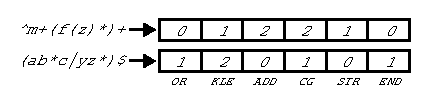
\includegraphics[height=0.6in]{nontex/illustrations/featureParsing.eps}
\caption{Two patterns parsed into feature vectors}
\label{fig:featureParsing}
\vspace{-12pt}
\end{figure}

Once all patterns were transformed into vectors, each feature was examined independently for all patterns, tracking the number of patterns, files and projects that the each feature appears in at least once.

\begin{table*}
\begin{center}
\begin{footnotesize}
\caption{Frequency of feature appearance in Projects, Files and Patterns, with number of tokens observed and the maximum number of tokens observed in a single pattern.}
\label{table:featureStatsOnly}
\begin{tabular}
{lllcccc  cc}
rank & code & example & \% projects & nProjects & nFiles & nPatterns & nTokens & maxTokens. \\ 
\toprule[0.16em]
1 & ADD & \begin{minipage}{0.5in}\begin{verbatim}z+\end{verbatim}\end{minipage} & 73.2 & 1,204 & 9,165 & 6,003 & 11,136 & 30 \\ 
\midrule
2 & CG & \begin{minipage}{0.5in}\begin{verbatim}(caught)\end{verbatim}\end{minipage} & 72.6 & 1,194 & 9,559 & 7,130 & 12,707 & 17 \\ 
\midrule
3 & KLE & \begin{minipage}{0.5in}\begin{verbatim}.*\end{verbatim}\end{minipage} & 66.8 & 1,099 & 8,163 & 6,017 & 11,620 & 50 \\ 
\midrule
4 & CCC & \begin{minipage}{0.5in}\begin{verbatim}[aeiou]\end{verbatim}\end{minipage} & 62.4 & 1,026 & 7,648 & 4,468 & 8,179 & 42 \\ 
\midrule
5 & ANY & \begin{minipage}{0.5in}\begin{verbatim}.\end{verbatim}\end{minipage} & 61.1 & 1,005 & 6,277 & 4,657 & 7,119 & 60 \\ 
\midrule
6 & RNG & \begin{minipage}{0.5in}\begin{verbatim}[a-z]\end{verbatim}\end{minipage} & 51.6 & 848 & 5,092 & 2,631 & 8,043 & 50 \\ 
\midrule
7 & STR & \begin{minipage}{0.5in}\begin{verbatim}^\end{verbatim}\end{minipage} & 51.4 & 846 & 5,458 & 3,563 & 3,661 & 12 \\ 
\midrule
8 & END & \begin{minipage}{0.5in}\begin{verbatim}$\end{verbatim}\end{minipage} & 50.3 & 827 & 5,393 & 3,169 & 3,276 & 12 \\ 
\midrule[0.12em]
9 & NCCC & \begin{minipage}{0.5in}\begin{verbatim}[^qwxf]\end{verbatim}\end{minipage} & 47.2 & 776 & 3,947 & 1,935 & 2,718 & 15 \\ 
\midrule
10 & WSP & \begin{minipage}{0.5in}\begin{verbatim}\s\end{verbatim}\end{minipage} & 46.3 & 762 & 4,704 & 2,846 & 6,128 & 32 \\ 
\midrule
11 & OR & \begin{minipage}{0.5in}\begin{verbatim}a|b\end{verbatim}\end{minipage} & 43 & 708 & 3,926 & 2,102 & 2,606 & 15 \\ 
\midrule
12 & DEC & \begin{minipage}{0.5in}\begin{verbatim}\d\end{verbatim}\end{minipage} & 42.1 & 692 & 4,198 & 2,297 & 4,868 & 24 \\ 
\midrule
13 & WRD & \begin{minipage}{0.5in}\begin{verbatim}\w\end{verbatim}\end{minipage} & 39.5 & 650 & 2,952 & 1,430 & 2,037 & 13 \\ 
\midrule
14 & QST & \begin{minipage}{0.5in}\begin{verbatim}z?\end{verbatim}\end{minipage} & 39.2 & 645 & 3,707 & 1,871 & 3,290 & 35 \\ 
\midrule
15 & LZY & \begin{minipage}{0.5in}\begin{verbatim}z+?\end{verbatim}\end{minipage} & 36.8 & 605 & 2,221 & 1,300 & 1,761 & 12 \\ 
\midrule
16 & NCG & \begin{minipage}{0.5in}\begin{verbatim}a(?:b)c\end{verbatim}\end{minipage} & 24.6 & 404 & 1,709 & 791 & 1,453 & 28 \\ 
\midrule
17 & PNG & \begin{minipage}{0.5in}\begin{verbatim}(?P<name>x)\end{verbatim}\end{minipage} & 21.5 & 354 & 1,475 & 915 & 2,399 & 16 \\ 
\midrule
18 & SNG & \begin{minipage}{0.5in}\begin{verbatim}z{8}\end{verbatim}\end{minipage} & 20.7 & 340 & 1,267 & 581 & 1,159 & 17 \\ 
\midrule
19 & NWSP & \begin{minipage}{0.5in}\begin{verbatim}\S\end{verbatim}\end{minipage} & 16.4 & 270 & 776 & 484 & 676 & 10 \\ 
\midrule
20 & DBB & \begin{minipage}{0.5in}\begin{verbatim}z{3,8}\end{verbatim}\end{minipage} & 14.5 & 238 & 647 & 367 & 573 & 11 \\ 
\midrule
21 & NLKA & \begin{minipage}{0.5in}\begin{verbatim}a(?!yz)\end{verbatim}\end{minipage} & 11.1 & 183 & 489 & 131 & 148 & 3 \\ 
\midrule
22 & WNW & \begin{minipage}{0.5in}\begin{verbatim}\b\end{verbatim}\end{minipage} & 10.1 & 166 & 438 & 248 & 408 & 36 \\ 
\midrule
23 & NWRD & \begin{minipage}{0.5in}\begin{verbatim}\W\end{verbatim}\end{minipage} & 10 & 165 & 305 & 94 & 149 & 6 \\ 
\midrule
24 & LWB & \begin{minipage}{0.5in}\begin{verbatim}z{15,}\end{verbatim}\end{minipage} & 9.6 & 158 & 281 & 91 & 107 & 3 \\ 
\midrule
25 & LKA & \begin{minipage}{0.5in}\begin{verbatim}a(?=bc)\end{verbatim}\end{minipage} & 9.6 & 158 & 358 & 112 & 133 & 4 \\ 
\midrule
26 & OPT & \begin{minipage}{0.5in}\begin{verbatim}(?i)CasE\end{verbatim}\end{minipage} & 9.4 & 154 & 377 & 231 & 238 & 2 \\ 
\midrule
27 & NLKB & \begin{minipage}{0.5in}\begin{verbatim}(?<!x)yz\end{verbatim}\end{minipage} & 8.3 & 137 & 296 & 94 & 117 & 4 \\ 
\midrule[0.12em]
28 & LKB & \begin{minipage}{0.5in}\begin{verbatim}(?<=a)bc\end{verbatim}\end{minipage} & 7.3 & 120 & 255 & 80 & 99 & 4 \\ 
\midrule
29 & ENDZ & \begin{minipage}{0.5in}\begin{verbatim}\Z\end{verbatim}\end{minipage} & 5.5 & 90 & 149 & 89 & 89 & 1 \\ 
\midrule
30 & BKR & \begin{minipage}{0.5in}\begin{verbatim}\1\end{verbatim}\end{minipage} & 5.1 & 84 & 129 & 60 & 73 & 4 \\ 
\midrule
31 & NDEC & \begin{minipage}{0.5in}\begin{verbatim}\D\end{verbatim}\end{minipage} & 3.5 & 58 & 92 & 36 & 51 & 6 \\ 
\midrule
32 & BKRN & \begin{minipage}{0.5in}\begin{verbatim}(P?=name)\end{verbatim}\end{minipage} & 1.7 & 28 & 44 & 17 & 19 & 2 \\ 
\midrule
33 & VWSP & \begin{minipage}{0.5in}\begin{verbatim}\v\end{verbatim}\end{minipage} & 0.9 & 15 & 16 & 13 & 14 & 2 \\ 
\midrule
34 & NWNW & \begin{minipage}{0.5in}\begin{verbatim}\B\end{verbatim}\end{minipage} & 0.7 & 11 & 11 & 4 & 5 & 2 \\ 
\bottomrule[0.13em]
\end{tabular}
\end{footnotesize}
\end{center}
\end{table*}


\subsection{Feature usage within the corpus}
Table~\ref{table:featureStatsOnly} displays feature usage from the corpus in terms of the number of patterns, files and projects, as well as in terms of tokens used.

The first column, \emph{rank}, lists the rank of a feature (relative to other features) in terms of the number of projects in which it appears. The next column, \emph{code}, gives a succinct reference string for the feature as described in Section~\ref{sec:featureDescriptions}. The \emph{example} column provides a short example of how the feature can be used.The next six columns contain usage statistics providing a variety of perspectives on how frequently the features are used in the observed population.

The \emph{\% projects} column contains the percentage of projects  using a feature out of the 1,645 projects scanned that contain at least one pattern in the corpus.  The \emph{nProjects} column provides the number of projects that contain at least one usage of a feature.  Assuming that one project generally corresponds to some high-level goal of a programmer or a team of programmers, these values provide a sense of how frequently a feature is \emph{part of a software solution} in even the slightest way.  Because of the generality of this measure and the goal of this study to gauge how features of regular expressions are used in general, these values are used to determine the rank of a feature.

The \emph{nFiles} column specifies the number of files that contain at least one observed usage of the feature.  For reference, recall that a total of \dbfetch{nFilesUsingRegex} files were scanned that contain at least one feature usage.  Assuming that programmers organize code into separate files based on what the code needs to do, this number can provide insight into the variety of different conceptually separate \emph{task categories} a feature is used for.

The \emph{nPatterns} column contains the number of patterns in which a feature was observed. Each regex is compiled from a particular pattern and performs at least one function desired by a programmer.  Therefore the number of patterns composed using a feature can provide insight into the number of \emph{specific tasks} a feature is used for.

The \emph{nTokens} column, gives the total number of tokens observed for a feature, combining the token counts of all patterns in the corpus.  This value provides a sense of how often the language feature is used \emph{for any task}.

The last column, \emph{maxTokens}, gives the maximum number of times that a feature appears in a single regex.  Assuming that a feature that a programmer finds convenient is used more frequently in a given regex, this value provides a sense of \emph{convenience} provided by the feature.
